\clearpage

\pagestyle{fancy}
\fancyhf{}
\renewcommand{\headrulewidth}{0pt}
\cfoot{\thepage}
\chead{\nouppercase{\sc Prologue}}

\phantomsection\section*{\hypertarget{prologue}{Prologue: Heston-NIG motivating relationships}}
\addcontentsline{toc}{section}{Prologue: Heston-NIG motivating relationships}

This prologue presents the author's personal account of the preliminary motivations behind this thesis. These originate primarily from a desire to validate, strengthen and generalise the main result of \cite{mechkov_2015}, after experiencing modelling benefits of this in financial risk management. Although not strictly required to appreciate the thesis's mathematical contributions, results and goals presented here will be referred to throughout the remainder.

\vspace{3mm}\textbf{Personal modelling experience.} I have worked as a quantitative analyst in risk management for nine years thus far, mostly at an advisory firm called JCRA, set up by John Rathbone in 1989 and bought by Chatham Financial in 2019. In 2015, a year before starting to work towards a PhD at Imperial College, I was reviewing models of financial variables (e.g.~interest rates, foreign exchange rates, stock prices) for the purpose of various simulation-based computations related to the possible future values of clients' derivative portfolios.

For this purpose, we had at our disposal Numerix's model library (Numerix is a trading and risk management technology provider, see e.g.~\href{https://www.numerix.com/}{Numerix.com}). This is how I came across Numerix's `fast-reversion Heston' (FRH) model, specifically when comparing calibration accuracies and stabilities of various foreign exchange (FX) models. The details of this are available in \cite{mechkov_2015}, and an implementation at \href{https://github.com/rmcrkd/frh-fx}{github.com/rmcrkd/frh-fx}.

It became clear that this FRH extension of the classical stochastic volatility model of \cite{heston_1993} was excellent for our purposes. In simple terms, this model can, like alternative extensions of the Heston model (e.g.~local-stochastic volatility or jump-diffusion), replicate the 100 or so quotes in an FX implied volatility surface with near-perfect accuracy, and it can also be easily simulated accurately, unlike its classical namesake. In my experience, it achieves this with relatively few, stable and physically meaningful parameters, the effects of which one stands a chance of explaining to non-mathematical colleagues and clients.

I was therefore surprised to find that this FRH model is not really a new model, but, at least in its basic form, a repackaged old one. Specifically, it is a reparameterised normal inverse-Gaussian (NIG) model from \cite{barndorff-nielsen_1997}, wherein the variable of concern, e.g.~FX rate or equity price, is modelled by an exponentiated NIG (exp-NIG) L\'evy process. Valuably, the influences of Heston's parameters on this FRH version are preserved, for which MSc graduates and quantitative analysts in general usually have strong intuition.

My immediate surprise originated from the fact that these apparently related Heston and NIG models are two of the most popular in finance, and so vast sums of companies' wealth, and their related decision making, depend on their properties. In my line of work, this dependence primarily manifests from what such models say about derivative values.

Mathematically, the models being related here exist in different frameworks. One depends inseparably on It\^o calculus, accommodating continuous sample paths like Heston's, and the other on non-Brownian L\'evy processes, with discontinuous paths like those of the NIG model. Popularity aside, these models are exemplars as good as any for these contrasting theoretical frameworks. Supplementing practical experiences, such theoretical considerations reinforce the value of developing a deeper understanding of the relationship between these two models.

\vspace{3mm}\textbf{Mechkov's Heston-NIG relationship.} The Heston and NIG relationship from \cite{mechkov_2015} is now summarised, presented in notation consistent with the core of this thesis. This is a relationship manifesting through limits of parameters, so consider a general family of classical Heston price processes $S^n=\{S^n_t\}_{t\in\RR_+}$, with $n>0$, exactly as in \cite{heston_1993},~
\begin{equation}\label{eq:heston_prologue}
    \dd V^n_t = \sigma_n\sqrt{V^n_t}\dd W^1_t + \kappa_n(\theta_n - V^n_t)\dd t,\quad \dd S^n_t = \sqrt{V^n_t}S^n_t\dd W^{\rho_n}_t,\quad (V^n_0,S^n_0) := (v_n,1),
\end{equation}
where $W^0,W^1$ are independent 1d Brownian motions starting at 0, and $W^{\rho_n}:=\sqrt{1-\rho_n^2}W^0+\rho_n W^1$. In finance, the stochastic differential equations (SDEs) which the variance processes $V^n=\{V^n_t\}_{t\in\RR_+}$ verify are called CIR SDEs, because of \cite{cox_1985}.

The parameters $\sigma_n,\kappa_n,\theta_n, v_n >0$ are respectively known as volatility of volatility, reversion speed, reversion level, and starting variance, and $\rho_n\in[-1,1]$ correlation. For some fixed $\sigma,\theta,v>0$ and $\rho\in[-1,1]$, now set $(\sigma_n,\kappa_n,\theta_n,\rho_n,v_n):=(n\sigma,n,\theta,\rho,v)$, so that $n$ indexes the reversion speeds of this family $\{S^n\}_{n>0}$, and \autoref{eq:heston_prologue} more simply reads
\begin{equation}\label{eq:heston_prologue2}
    \dd V^n_t = n\sigma\sqrt{V^n_t}\dd W^1_t + n(\theta - V^n_t)\dd t,\quad \dd S^n_t = \sqrt{V^n_t}S^n_t\dd W^{\rho}_t,\quad (V^n_0,S^n_0) := (v,1).
\end{equation}
The fact that \emph{both} the diffusive and reversionary components of the CIR SDEs for each $V^n$ here scale linearly with $n$, so grow at the same rate as $n\to\infty$, is critical to the novelty of this parameterisation, and the resulting NIG relationship. This differs from that considered extensively in \cite{fouque_2011} and preceding articles by the same authors where, in the same notation here, one would instead set $\sigma_n:=\sqrt{n}\sigma$.

When defining L\'evy processes, it is sufficient and common to state their marginal characteristic function, and the NIG one can be found, alongside Heston's, in \cite{mechkov_2015}. But following \cite{applebaum_2009}, it is possible and informative to construct an exp-NIG process $S^0=\{S^0_t\}_{t\in\RR_+}$ from the same Brownian motions $W^0,W^1$ as in \autoref{eq:heston_prologue2}, by
\begin{equation}\label{eq:nig_prologue}
    S^0_t := \exp\left(\sqrt{1-\rho^2}W^0_{X^0_t} + \frac{2\rho-\sigma}{2\sigma}X^0_t -\frac{\rho\theta}{\sigma} t\right),\quad X^0_t:=\inf\bigg\{x>0:x-\sigma W^1_x > \theta t\bigg\}.
\end{equation}
The process $X^0=\{X^0_t\}_{t\in\RR_+}$ is an inverse-Gaussian (IG) subordinator, which is a non-decreasing L\'evy process. The main result of \cite{mechkov_2015} can now be stated as follows.
\begin{theorem}[Mechkov's Heston-NIG relationship]\label{thm:mech_pro}
    Let $\{S^n\}_{n>0}$ be the family of Heston price processes from \autoref{eq:heston_prologue2}, and $S^0$ the exponentiated NIG process from \autoref{eq:nig_prologue}. Then for each fixed $t\in\RR_+$, the convergence in distribution $S^n_t\cd S^0_t$ takes place as $n\to\infty$.
\end{theorem}

At first this result can seem related to the relationship known earlier between the distribution of a \emph{fixed} Heston process at large times and the NIG distribution, established independently in \cite{keller-ressel_2011} and \cite{forde_2011}. However, when one tries to map this large-time result onto parameters of a \emph{family} of Heston models (through scaling properties of Brownian motion), the resulting family is not quite like those in \autoref{eq:heston_prologue2}, but those obtained when instead setting $(\sigma_n,\kappa_n,\theta_n,\rho_n,v_n):=(n\sigma,n,n\theta,\rho,nv)$ in \autoref{eq:heston_prologue}.

With these starting variances and reversion levels additionally exploding as $n\to\infty$, the resulting distribution of the family $S^n$ at any fixed time grows in a manner which cannot be reconciled with those of a fixed exp-NIG process. So these earlier large-time results for a fixed Heston model cannot be adapted to a relationship with a fixed limiting model. Indeed, the authors concluded this at the time, which now emphasises the novelty of \autoref{thm:mech_pro}.

\vspace{3mm}\textbf{The volatility skew paradox.} With \autoref{thm:mech_pro} stated, it is worth highlighting a paradox of sorts which it raises. Around the time when I became aware of and had computationally verified Mechkov's Heston-NIG relationship, I also became aware of the preprint of \cite{gatheral_2018} and the growing popularity of `rough' volatility models. These models usually extend a classical counterpart like Heston's, and are distinguished by the depending volatility or variance process having a comparably low H\"older regularity. So these processes look rough, like fractional Brownian motion with a low Hurst parameter.

In my area of derivative-related work, such models are supported by their ability to reproduce observed `implied volatility skews' in equity markets. First demonstrated in \cite{bayer_2016}, this is backed up by the theory of \cite{alos_2007} and \cite{fukasawa_2011}. For a price process $S=\{S_t\}_{t\in\RR_+}$ and future time, this skew is loosely related, via some transformations, to the third moment of $S_t$. See \cite{bergomi_2016} or \autoref{eq:skew_curv}.

The theory says that the classical Heston and NIG models featuring in \autoref{thm:mech_pro} will respectively \emph{under} and \emph{over}-emphasise how a skew consistent with rough volatility evolves backwards in time, towards $t=0$. The theoretical justification of this for the NIG model is in \cite{gerhold_2016}. But a consequence of \autoref{thm:mech_pro} is that the implied volatilities from these models, from which skews derive, will \emph{converge} as $n\to\infty$. This is demonstrated graphically in \cite{mechkov_2015}, and we reproduce something similar in \autoref{fig:vols_converge}. So how can this under and over-emphasis be explained, in light of this convergence?

\begin{figure}[ht]
    \centering
    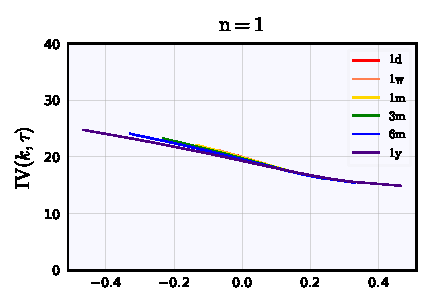
\includegraphics[width=0.50\linewidth]{figures/surface_converge_n1}
    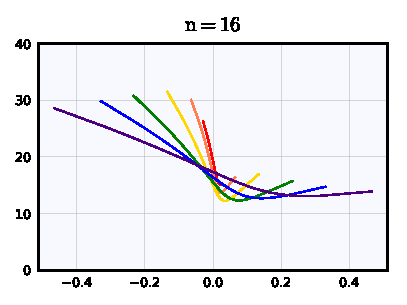
\includegraphics[width=0.47\linewidth]{figures/surface_converge_n16}

    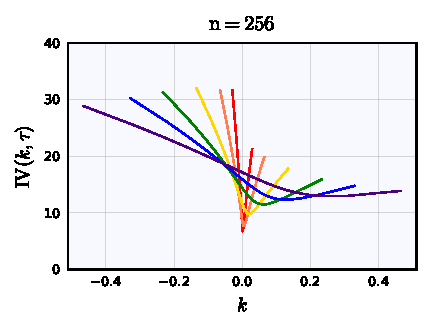
\includegraphics[width=0.50\linewidth]{figures/surface_converge_n256}
    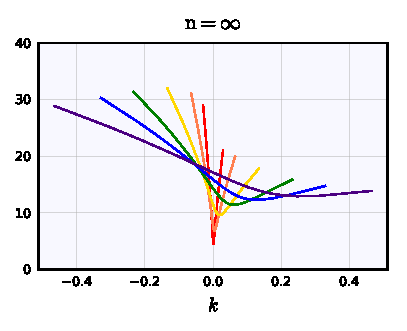
\includegraphics[width=0.47\linewidth]{figures/surface_converge_ninf}
    \caption{Like in \cite{mechkov_2015}, implied volatilities IV$(k,\tau)$ from the Heston model in \autoref{eq:heston_prologue2}, with $n=1,16,256$, are shown to converge across logstrikes $k$ to those of the NIG model ($n=\infty$) from \autoref{eq:nig_prologue}. This is a consequence of \autoref{thm:mech_pro}. Maturities $\tau$ range from a day ($\tau=1/256$) to a year ($\tau=1$), and $\sigma\!=\!0.2$, $\theta\!=\!v\!=\!0.04$, $\rho\!=\!-0.7$.}
    \label{fig:vols_converge}
\end{figure}

Despite few being aware of \autoref{thm:mech_pro} and its consequences, this paradox is actually understood, especially by practitioners, many of whom do not see a problem. A resolution is provided in \cite{bergomi_2016}, and the fact there is one is because these theoretical under and over-emphasis statements sometimes only apply with a meaningful degree of accuracy over an impractically short timescale, possibly even where no observable data exists.

As in \cite{bergomi_2016}, practitioners like this author have long been successfully bypassing needs for rough volatility models by foremost employing fast reversion speeds in classical models. A theoretical relationship between rough and fast reverting models was later revealed by certain representations of rough processes which show they depend implicitly on \emph{arbitrarily} large reversion speeds, see e.g.~\cite{muravlev_2011} and \cite{abijaber_2019b}. This dependence is just carefully controlled, in a manner which does not produce jumps like those present in the NIG limit of \autoref{thm:mech_pro}, but instead just reduces paths' H\"older regularity. Following private discussions, the presentation \cite{abijaber_2019a} was the first to expose this link between rough volatility and jumps, via different reversionary properties.

The point here is \emph{not} about precise reproductions of skews, which I sincerely believe is done best by rough volatility models, at least in the equity markets. It is about where we collectively place our research focus, and the value of it. Having co-written \cite{mccrickerd_2018} on derivative pricing for a particular rough volatility model, I felt like I had spent as much time as anyone treating practical difficulties associated with rough volatility models, especially regarding \emph{simulation}, and as a result was ready to consider alternatives.

Although simulation of the Heston price process $S^n$ from \autoref{eq:heston_prologue2} becomes more difficult as the reversion speed $n$ is raised, justifying various approximation techniques like those of \cite{andersen_2008}, the exp-NIG limit $S^0$ as $n\to\infty$ in \autoref{thm:mech_pro} can be simulated exactly. As already noted, fast reversion speeds in classical models are being relied upon in practice, as an alternative to rough volatility. See e.g.~\cite{bergomi_2016} and \cite{decol_2013} for calibrated values of the order of 1,000\% deriving respectively from equity and FX derivative price data, but note \cite{fouque_2011} obtain values as high as 10,000\% from realised data, still corresponding to a plausible reversionary timescale of 2--3 trading days.

Given positive personal experiences with the FRH model, and that the Heston-NIG relationship from \autoref{thm:mech_pro} can help to alleviate \emph{both} of these volatility skew and simulation problems, it seemed clear that I, if not others also, should first spend more time trying to better understand this surprising new fast reversion relationship between these relatively simple existing models, before seriously reconsidering rough volatility models again.

This version of Occam's razor is particularly salient in finance, because regulators often neglect the complexity of output requested from companies. The requirement to compute valuation adjustments (XVAs) demonstrates this. These depend on the future values of derivative portfolios mentioned earlier, and are what led me to Numerix's FRH model. At JCRA, we used this model for FX XVAs for five years, because it consistently calibrates well to FX implied volatility surfaces, and can be simulated efficiently and exactly thereafter.

\vspace{3mm}\textbf{The general preliminary goal.} In the knowledge of \autoref{thm:mech_pro} and some of its consequences, the distant goal was to strengthen and generalise this, to widen the applicability from practitioners relying on the Heston and NIG models like me to those relying on others.

It was not immediately clear how to generalise \autoref{thm:mech_pro}, so strengthening it appeared to be the better starting point, with the hope that a stronger understanding of it would later reveal how to generalise. Towards this strengthening, notice that while Mechkov's relationship in \autoref{thm:mech_pro} references Heston and NIG \emph{models}, unlike the earlier large-time connection, it is still not a relationship between them. Rather, it should be considered a family of relationships, between the random variables $\{S^n_t\}_{n\ge0}$ relating to each fixed time.

Nevertheless the convergence $S^n_t\cd S^0_t$ for a fixed time is valuable in practice, because from it we obtain $\EE[\#(S^n_t)]\to\EE[\#(S^0_t)]$ for sufficiently-behaved functions $\#:\RR\to\RR$. As covered in \autoref{sec:martingale}, such a function $\#$ and values like $\EE[\#(S^0_t)]$ can be related to derivative payoffs and prices respectively, under some sensible assumptions. So this convergence tells us how a class of `European' derivative prices will behave in the limit of \autoref{thm:mech_pro}. Indeed, letting $\#$ correspond to a particular (put option) derivative, this confirms the convergence of Heston's implied volatilities to those of the NIG model, as demonstrated in \autoref{fig:vols_converge}.

To widen the applicability to other common, path-dependent, derivatives, we require $\EE[\#(S^n)]\to\EE[\#(S^0)]$ with $\#$ now generalising to a suitably-behaved function from a set $\cX$ of \emph{paths} containing those of $S^n$ and $S^0$. This is provided, almost by definition, by the weak convergence $S^n\cw S^0$ on a metric space $(\cX,d_\cX)$, where $\#:(\cX,d_\cX)\to(\RR,d_\RR)$ must in general be bounded and continuous, and $d_\RR$ can be taken as the usual Euclidean metric on $\RR$.

Taking this deeper, if we want to understand how derivative payoffs $\#(S^n)$ relate to those of $\#(S^0)$, not just resulting prices hidden behind expectations (i.e.~integrals), we require stronger notions of convergence $S^n\xrightarrow{n\to\infty} S^0$ still, say those of convergence in probability or almost sure (a.s.). Understanding whether this is actually possible is intimately connected to whether the Brownian motions $W^0,W^1$ in both \autoref{eq:heston_prologue2} and \autoref{eq:nig_prologue} are related.

To emphasise difficulties in obtaining these goals, it is worth providing a spoiler. Despite the relevant set $\cX$ of \emph{c\`adl\`ag} paths containing those of both Heston and NIG models, it turns out even weak convergence $S^n\cw S^0$ is violated on all Skorokhod metric spaces. From \cite{skorokhod_1956}, these spaces appear often in financial stochastic process limit theorems.

There is thankfully a recipe for establishing weak convergence, sometimes called `Prokhorov's approach' after \cite{prokhorov_1956}, summarised well in \cite{jacod_2003} and depending on something called `tightness'. But this does not say what to do when things go wrong; when tightness is violated. Unfortunately this is the setting we are in here, despite working with some of the most popular, and relatively simple, models. Indeed, much of my research originated from a need for a different approach to stochastic process limit theorems.

As the title of this thesis suggests, the focus has shifted away from these preliminary goals. It has become about the mathematics developed to obtain them, about a change of perspective on the Heston model, moving away from a dependence on It\^o calculus in favour of random ODEs, and about a resulting robust modelling framework which accommodates generalisations of this Heston and NIG relationship, and eventually rough volatility as well.

Answers to specific questions here relating to classical Heston models are found in \autoref{sec:price_limits}, where a surprising \emph{interval-valued} generalisation $S^\bullet$ of the NIG process must be introduced,~
\begin{equation}\label{eq:ex_nig_pro}
    X^0_t:=\inf\bigg\{x>0:x-\sigma W^1_x > \theta t\bigg\},\quad S^\bullet_t := \bigg\{\exp\left(W^\rho_x - \frac12 x\right) : x\in[X^0_{t_-},X^0_t] \bigg\}.
\end{equation}
This has a beautifully intimate relationship with the standard NIG process from \autoref{eq:nig_prologue}, which can actually be expressed more compactly as $S^0_t = \exp(W^\rho_{X^0_t} - \frac12 X^0_t)$. The \hyperlink{epilogue}{Epilogue} focuses in on the \emph{origin} of the resulting weak convergence, and is presented from the accessible perspective of It\^o SDEs. There, relationships between the CIR process and several L\'evy processes connected with $X^0$ are established on a new `exit-time' metric space.
